\documentclass{myhw}
\linespread{1.05}        % Palatino needs more leading (space between lines)
\usepackage{extarrows}
\usepackage{mathrsfs}
\usepackage{braket}
\usepackage{amsmath}
\usepackage{listings}

\titleformat{\section}[runin]{\sffamily\bfseries}{}{}{}[]
\titleformat{\subsection}[runin]{\sffamily\bfseries}{}{}{}[]
\renewcommand{\exname}{Question }
\renewcommand{\subexcounter}{(\alph{homeworkSectionCounter})}
\newcommand{\id}{\text{Id}}
\newcommand{\tr}{\text{Tr}}
\newcommand{\rib}{\text{Rib}}

\title{CSC 2516 Homework 1}

\begin{document}

%% Question 1
\begin{homeworkProblem}
\textbf{Hard-Coding Networks.}
%%% Subquestion 1
\begin{homeworkSection}
\textbf{Verify Sort.} 
\emph{Find a set of weights and biases for a multilayer perceptron which determines if a list of length 4 is in sorted order.} \\
\\
$\textbf{W}^{(1)} = \begin{bmatrix}
-1 & 1 & 0 & 0\\
0 & -1 & 1 & 0\\
0 & 0 & -1 & 1
\end{bmatrix} \quad 
\textbf{b}^{(1)} = \begin{bmatrix} 0 \\ 0 \\ 0 \end{bmatrix} \quad 
w^{(2)} = \begin{bmatrix} 1 & 1 & 1 \end{bmatrix} \quad b^{(2)} = -3$
\end{homeworkSection}
%%% Subquestion 2
\begin{homeworkSection}
\textbf{Perform Sort.}
\emph{Describe how to implement a function $\hat{f} : \mathbb{R}^4 \rightarrow \mathbb{R}$ where $\hat{f} (x_1, x_2, x_3, x_4) = (\hat{x}_1, \hat{x}_2, \hat{x}_3, \hat{x}_4)$ where $(\hat{x}_1, \hat{x}_2, \hat{x}_3, \hat{x}_4)$ is $(x_1, x_2, x_3, x_4)$ in sorted order. Implement $f$ using a feedforward or recurrent neural network with element wise activations.} \\
\\
Bubble sort approach. \\
1. Make a min-max net. If input is A and B, $min = A - (A-B)_+, max = A + (B-A)_+$. Min-max net can be used to swap disordered numbers. \\
2. Given N inputs, construct $(N-1)!$ hidden layers, which all consist of the same number of outputs as the input layer. Each layer compares two neighboring inputs and swaps them if disordered. The order of comparison is as in the bubble sort. Specifically, the first two numbers are first compared, then, the second and the third, and so on. After the first round sorting from left to right, the last output will become the maximum value, and the second to last will become the second largest value. 
\\
\\
Brute-force approach. \\
In previous section, we get Verify Sort network, named $vs(\cdot)$. \\ 
1. Make permutations of the input. Assuming the number of input is $N$, we need $\mathbb{A}_N^N = N!$ permutations. The permutations are generated on the first hidden layer. Each node on the first hidden layer is only connected to the corresponding node on the input layer. For example, to generate a permutations $(\tilde{x}_1, \tilde{x}_2, \tilde{x}_3, \tilde{x}_4) = (x_2, x_3, x_1, x_4)$, the four nodes on the upper layer can only be connected to node $(\tilde{x}_1, \tilde{x}_2, \tilde{x}_3, \tilde{x}_4)$ respectively, i.e. only their weights are 1. \\
2. Verify sort. Employ Verify Sort network on all the permutations. We get $N!$ verification results, $vs(\tilde{x}_1, \tilde{x}_2, \tilde{x}_3, \tilde{x}_4)$. At the same time, we save the sum of all the verification results, $V = \sum vs(\tilde{x}_1, \tilde{x}_2, \tilde{x}_3, \tilde{x}_4)$, in case of duplicate input (if no duplicate input, $V = 1$).\\
3. Multiply verification results and original input, $\hat{f}(x_1, x_2, x_3, x_4) = \frac{\sum_{\tilde{x}_1, \tilde{x}_2, \tilde{x}_3, \tilde{x}_4}( (\tilde{x}_1, \tilde{x}_2, \tilde{x}_3, \tilde{x}_4) \times vs(\tilde{x}_1, \tilde{x}_2, \tilde{x}_3, \tilde{x}_4))}{\sum_{\tilde{x}_1, \tilde{x}_2, \tilde{x}_3, \tilde{x}_4}( (\tilde{x}_1, \tilde{x}_2, \tilde{x}_3, \tilde{x}_4)}$.
\end{homeworkSection}
%%% Subquestion 3
\begin{homeworkSection}
\textbf{Universal Approximation Theorem.}
\paragraph{1.3.1} 
\emph{Consider a bump function $g(h,a,b,x)=h \cdot \mathbb{I} (a \leq x \leq b)$ visualized in Figure 2. Given some $(h, a, b)$ show $\exists \tau : \hat{f_\tau}(x)=g(h,a,b,x)$.} \\
\\
n = 2 \quad
$\textbf{W}_0 = \begin{bmatrix} 1\\ -1 \end{bmatrix} \quad 
\textbf{b}_0 = \begin{bmatrix} -a \\ b \end{bmatrix} \quad 
\textbf{W}_1 = \begin{bmatrix} h & h \end{bmatrix} \quad \textbf{b}_1 = -h$
\paragraph{1.3.2} 
\emph{Given $f(x) = -x^2 + 1$ where where $I=[-1,1]$ and some initial function $\hat{f_0}(x)=0$ which is identically 0, construct a new function $\hat{f_1}(x) = \hat{f_0}(x) + g(h_1, a_1, b_1, x)$ such that $||f - \hat{f_1}|| < ||f - \hat{f_0}||$. Note that $h_1, a_1$, and $b_1$ are going to depend on our choice of $f, \hat{f_0}$ and $I$. Plot f and $\hat{f}_1$. } \\
\\
$f(x)=-x^2 + 1$. \\
\\
$\hat{f_1}(x) = \hat{f_0}(x) + g(h_1, a_1, b_1, x) = g(h_1, a_1, b_1, x)$. I set $h_1=\frac{3}{4}, a_1=-\frac{1}{2}, b_1=\frac{1}{2}$, $\hat{f_1}(x) = g(\frac{3}{4}, -\frac{1}{2}, \frac{1}{2}, x)$. \\
\\
Figure \ref{fig:q1.1} shows the figure of $f$, $\hat{f}_0$ and $\hat{f}_1$.
\begin{figure}[ht]
  \centering
  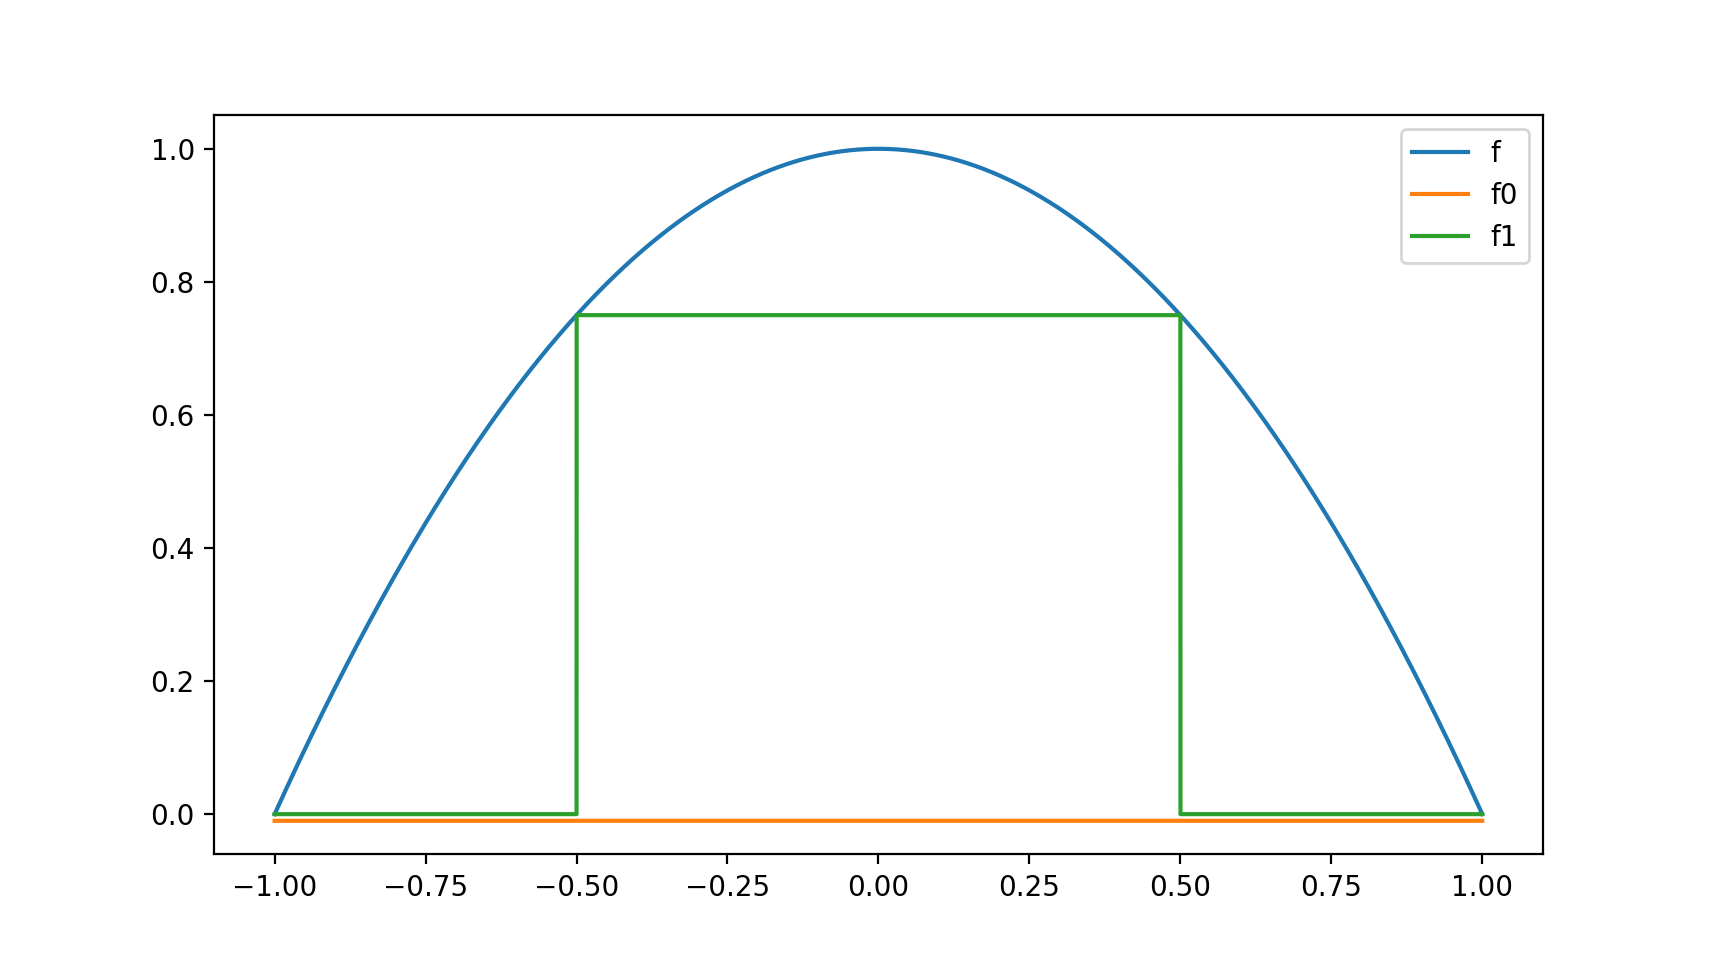
\includegraphics[width=.8\textwidth]{a1.png} 
  \caption{Figure of $f$, $\hat{f}_0$ and $\hat{f}_1$}
  \label{fig:q1.1}
\end{figure}
\paragraph{1.3.3} 
\emph{Describe a procedure which starts with $\hat{f_0}(x) = 0$ and a fixed $N$ then construct a series $\{\hat{f_i}\}_{i=0}^N$ where $\hat{f}_{i+1}(x) = \hat{f_i}(x) + g(h_{i+1}, a_{i+1}, b_{i+1}, x)$ which satisfies $||f - \hat{f}_{i+1}|| < ||f - \hat{f_i}||$. Plot $f, \hat{f_1}, \hat{f_2}$, and $\hat{f_3}$.} \\
\\
As we should construct $N$ functions, I first equally divide $[-1,0]$ into $(N+1)$ parts, 
\begin{gather*}
[-1, -1 + \frac{1}{N+1}], ..., [-1 + \frac{1}{N+1} * (k-1), -1 + \frac{1}{N+1} * k], ..., [-\frac{1}{N+1}, 0]
\end{gather*}
Thus, 
\begin{gather*}
\begin{aligned}
& a_{k+1} = -1 + \frac{k+1}{N+1} , \quad b_{k+1} = 1 - \frac{k+1}{N+1}, \\ 
h_{k+1} & = - (1-\frac{k+1}{N+1})^2 + 1 - \sum_{i=1}^{k} h_i = - (1-\frac{k+1}{N+1})^2 + 1 - \sum_{i=1}^{k} [- (1-\frac{i}{N+1})^2 + 1] \\
&= - (1-\frac{k+1}{N+1})^2 + 1 - (- (1-\frac{k}{N+1})^2 + 1) = (1-\frac{k}{N+1})^2 - (1-\frac{k+1}{N+1})^2
\end{aligned}
\end{gather*}
Suppose $N = 3$,
\begin{gather*}
\begin{aligned}
f(x) &= - x^2 + 1 \\
\hat{f_0}(x) &= 0 \\
\hat{f_1}(x) &= \begin{cases} \frac{7}{16} & -\frac{3}{4} \leq x \leq \frac{3}{4} \\ 0 & \text{otherwise} \end{cases} \\
\hat{f_2}(x) &= \begin{cases} \frac{5}{16} & -\frac{1}{2} \leq x \leq \frac{1}{2} \\ 0 & \text{otherwise} \end{cases} \\ 
\hat{f_3}(x) &= \begin{cases} \frac{3}{16} & -\frac{1}{4} \leq x \leq \frac{1}{4} \\ 0 & \text{otherwise} \end{cases} \\
\end{aligned}
\end{gather*}
Figure \ref{fig:q1.2} shows the figure of $f, \hat{f_1}, \hat{f_2}$, and $\hat{f_3}$.
\begin{figure}[ht]
  \centering
  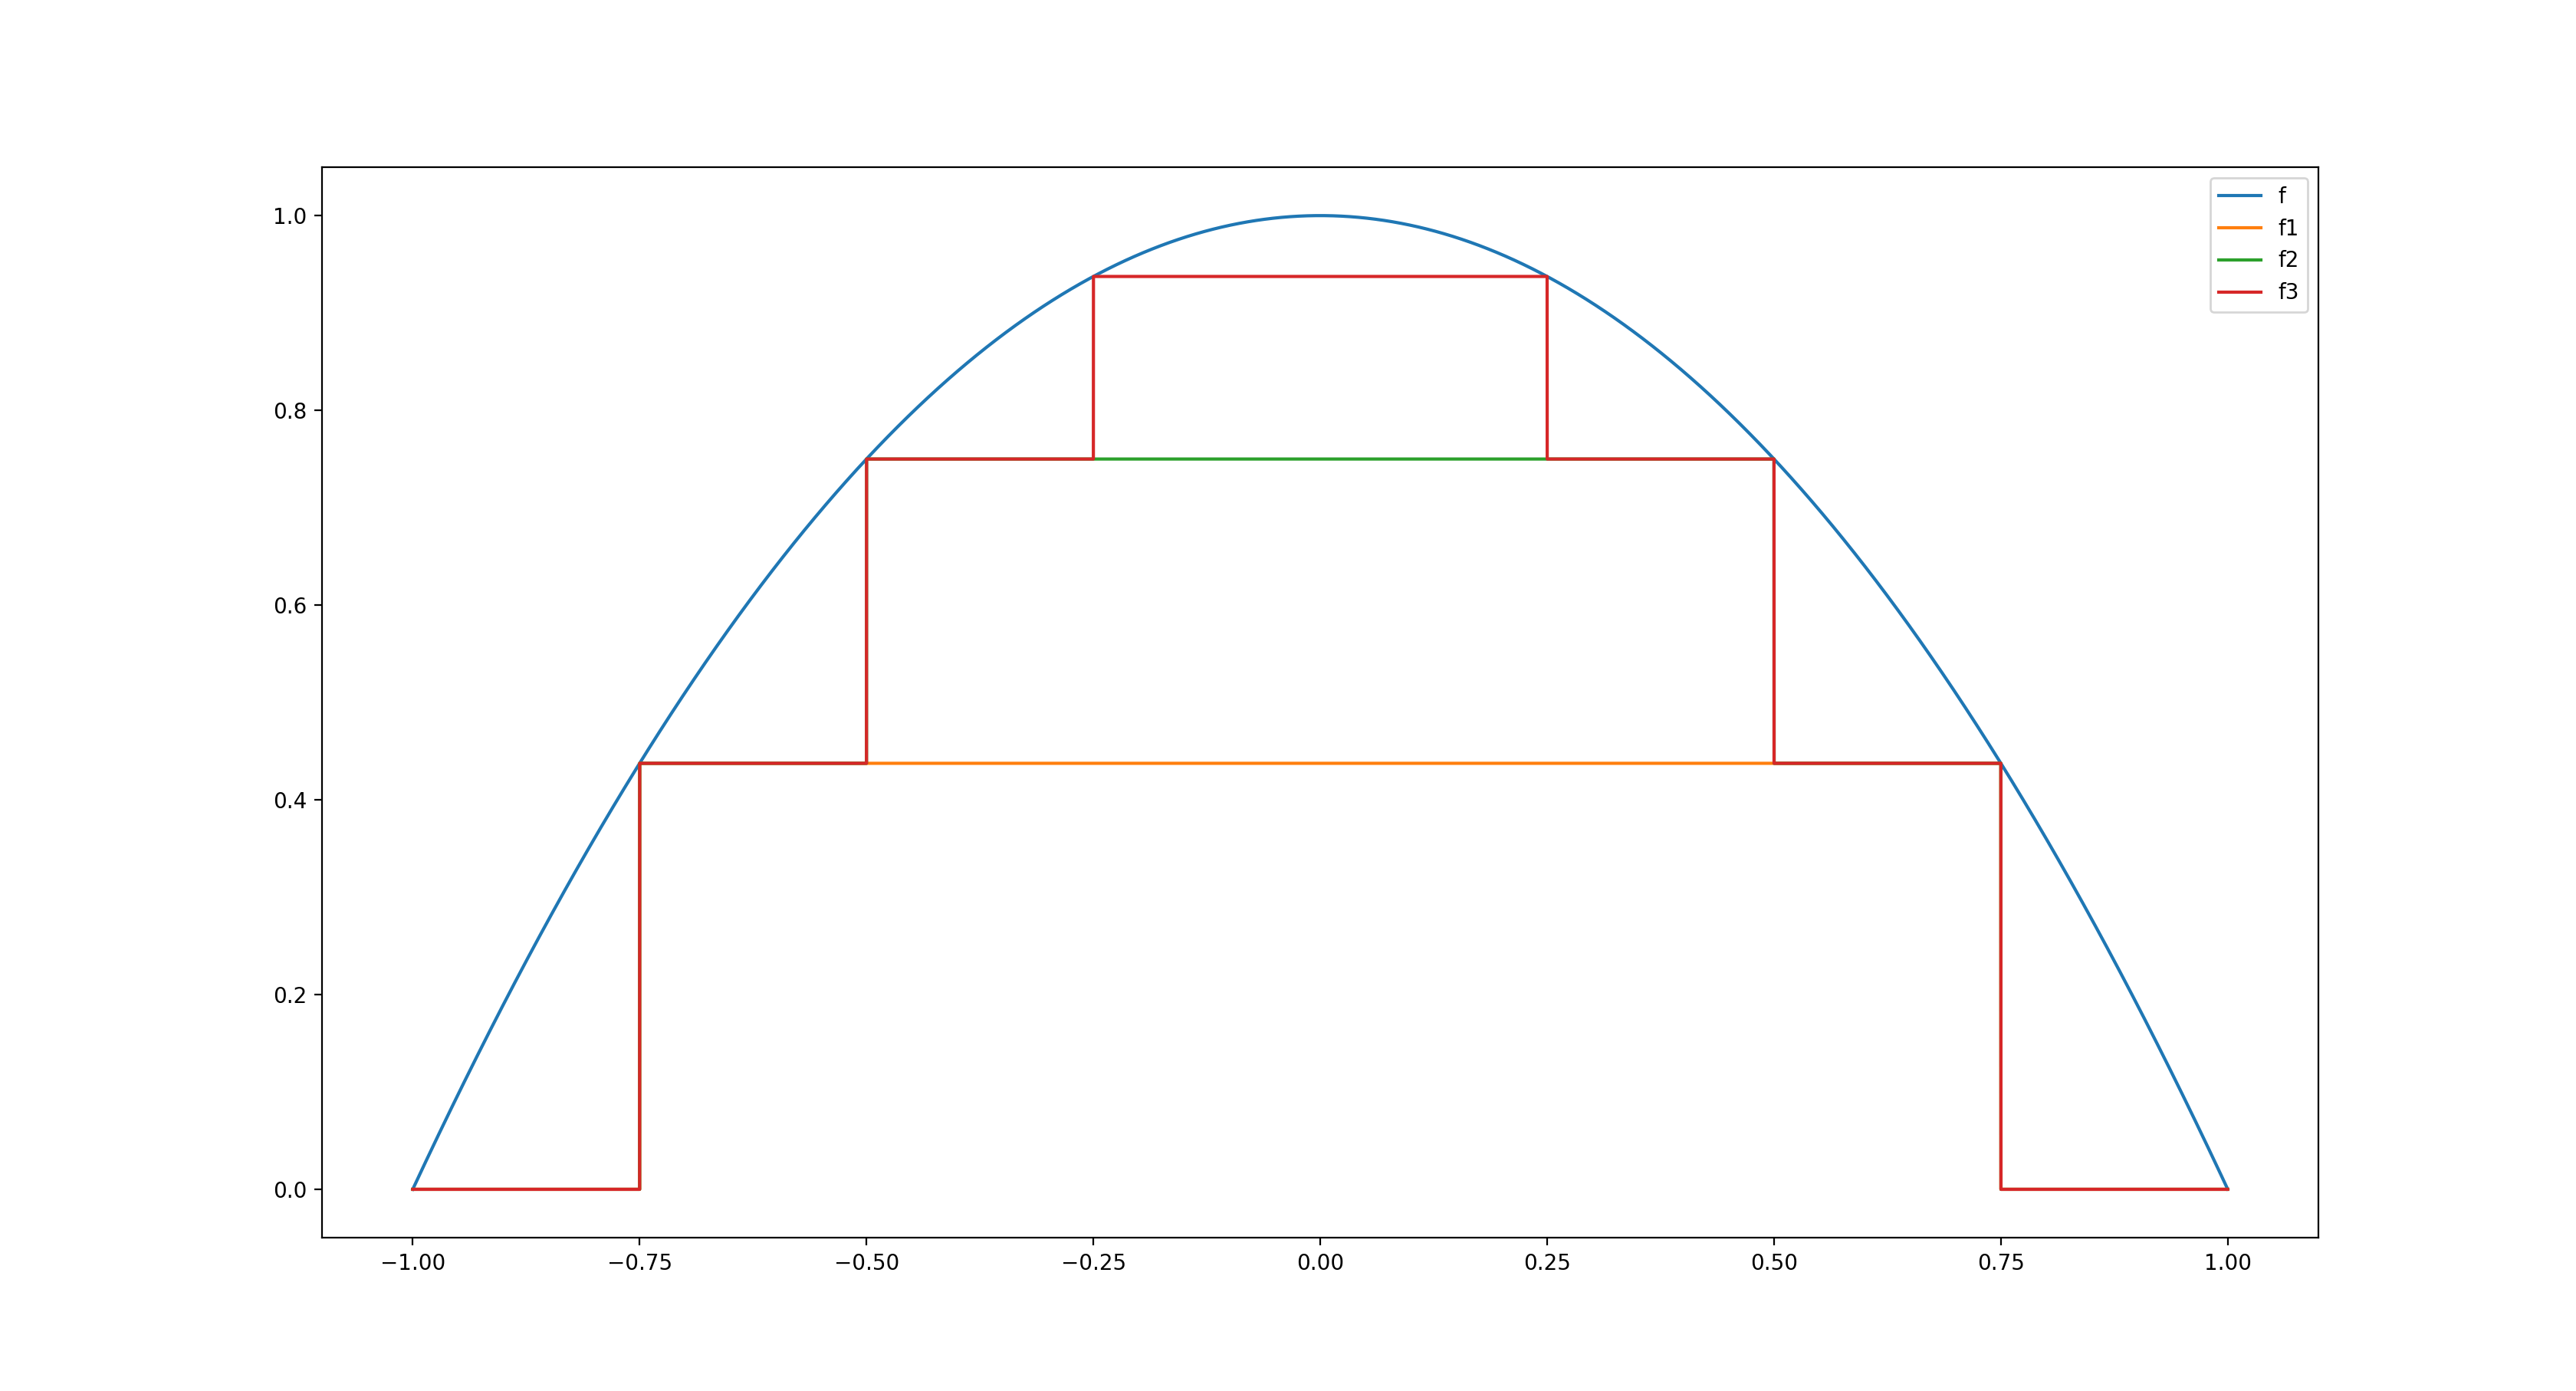
\includegraphics[width=\textwidth]{a1_2.png} 
  \caption{Figure of $f, \hat{f_1}, \hat{f_2}$, and $\hat{f_3}$}
  \label{fig:q1.2}
\end{figure}
\end{homeworkSection}
\end{homeworkProblem}


%% Question 2
\begin{homeworkProblem}
\textbf{Backprop.}
%%% Subquestion 1
\begin{homeworkSection} \textbf{Computational Graph.} \emph{Consider a neural network with N input units, M output units, and K hidden units.} 
\paragraph{2.1.1} \emph{Draw the computation graph relating $\textbf{x}, t, \textbf{z}, \textbf{h}, \textbf{y}, \textbf{y}', \textbf{r}, R, S,$ and $J$.} \\
\\
Figure \ref{fig:q2.1} shows the figure of the computation graph.
\begin{figure}[ht]
  \centering
  
\includegraphics[width=0.5\textwidth]{a2.eps} 
  \caption{Figure of computation graph relating $\textbf{x}, t, \textbf{z}, \textbf{h}, \textbf{y}, \textbf{y}', \textbf{r}, R, S,$ and $J$.}
  \label{fig:q2.1}
\end{figure}
\paragraph{2.1.2} \emph{Derive the backprop equations for computing $\bar{x} = \frac{\partial J}{\partial x}$. You may use softmax' to denote the derivative of the softmax function (so you don't need to write it out explicitly).} \\
\begin{gather*}
\begin{aligned}
\bar{J} &= 1 \\
\bar{R} &= \bar{S} = \bar{J} = 1 \\
\bar{y'} &= \bar{S} = 1 \\
\bar{y} &= \bar{y'} \cdot softmax'(y) = softmax'(y) \\
\bar{h} &= \bar{R} \cdot r + W^{(2)T} \bar{y} = r + W^{(2)T} softmax'(y) \\
\bar{z} &= \bar{h} \cdot ReLU'(z) = \begin{cases} \bar{h} &z>0 \\ 0 &otherwise \end{cases} \\
\bar{x} &= W^{(1)T} \bar{z} + \bar{y} = W^{(1)T} ( (r + W^{(2)T} softmax'(y)) \cdot ReLU'(z) ) + softmax'(y)
\end{aligned}
\end{gather*}
\end{homeworkSection}
%%% Subquestion 2
\begin{homeworkSection} \textbf{Vector-Jacobian Products (VJPs).}
\paragraph{2.2.1}
Compute $J \in \mathbb{R}^{n\times n}$ for $n=3$ and $v^T=[1,2,3]$ - i.e, weite down the values in $J=\begin{pmatrix} j_{1,1} & j_{1,2} & ... & j_{1,n}\\ j_{2,1} & j_{2,2} & ... & j_{2,n}\\ ... & ... & ... & ... \\ j_{n,1} & j_{n,2} & ... & j_{n,n} \end{pmatrix}$. 
\begin{gather*}
\begin{aligned}
J = \frac{\partial f}{\partial x} =\begin{pmatrix} 1 & 2 & 3 \\ 2 & 4 & 6 \\ 3 & 6 & 9 \end{pmatrix}
\end{aligned}
\end{gather*}
\paragraph{2.2.2}
\emph{What is the time and memory cost of evaluating the Jacobian of function $\textbf{f}$ in terms of $n$?}
\begin{gather*}
\begin{aligned}
J = \frac{\partial f}{\partial x} = v v^T
\end{aligned}
\end{gather*}
Thus, the time complexity of computing Jacobian is $\textbf{O}(n^2)$. 
Space complexity is also $\textbf{O}(n^2)$. 
\paragraph{2.2.3}
\emph{Describe how to evaluate $J^Ty$ with a time and memory cost that is linear in n. Then, compute $z=J^Ty$ where $v^T=(1,2,3)$ and $y^T=[1,1,1]$ - i.e., write down the entries in $z^T=[z_1, ..., z_n]$.} 
\begin{gather*}
\begin{aligned}
J^Ty = v v^T y = v (v^T y)
\end{aligned}
\end{gather*}
We could first calculate $v^Ty$, the time and space complexity of which is both $\textbf{O}(n)$; then, multiply $v$ with this scaler $v^Ty$ to get final result, which has the same time and space complexity as last process. \\
\\
For $v^T=(1,2,3)$ and $y^T=[1,1,1]$, 
\begin{gather*}
\begin{aligned}
z = J^Ty = v v^T y = v (v^T y) = 
\begin{bmatrix} 1 \\ 2 \\ 3 \end{bmatrix} (\begin{bmatrix} 1 \quad 2 \quad 3 \end{bmatrix} \begin{bmatrix} 1 \\ 1 \\ 1 \end{bmatrix}) = 6 \begin{bmatrix} 1 \\ 2 \\ 3 \end{bmatrix} = \begin{bmatrix} 6 \\ 12 \\ 18 \end{bmatrix}
\end{aligned}
\end{gather*}
\end{homeworkSection}
\end{homeworkProblem}


%% Question 3
\begin{homeworkProblem}
\textbf{Linear Regression.}
%%% Subquestion 1
\begin{homeworkSection}
\textbf{Deriving the Gradient.} 
\emph{Write down the gradient of the loss w.r.t. the learned parameter vector $\hat{w}$.} 
\begin{gather*}
\begin{aligned}
\frac{\partial L}{\partial \hat{w}} &= \frac{\partial \frac{1}{n} (X\hat{w} - t)^2}{\partial \hat{w}} = \frac{2}{n} X^T (X\hat{w} - t) = \frac{2}{n} (X^TX\hat{w} - X^Tt) \\
or \quad \frac{\partial L}{\partial \hat{w}} &= \frac{\partial \frac{1}{n} \sum_{i-1}^n (\hat{w}^T x^{(i)} - t^{(i)})^2}{\partial \hat{w}} = \frac{2}{n} \sum (\hat{w}^T x^{(i)} - t^{(i)}) x
\end{aligned}
\end{gather*}
\end{homeworkSection}
%%% Subquestion 2
\begin{homeworkSection}
\textbf{Underparameterized Model.}
\paragraph{3.2.1} \emph{First consider the underparamerized $d < n$ case. Write down the solution obtained by gradient descent assuming training converges. Show your work. Is the solution unique?}
\begin{gather*}
\begin{aligned}
X^TX\hat{w} - X^Tt &= 0 \\
\hat{w} &= (X^TX)^{-1} X^Tt
\end{aligned}
\end{gather*}
It is unique, as the answer above is calculated by setting vectorized gradient to 0. As a concave function, there should be only one lowest point.
\paragraph{3.2.2} \emph{Assume that ground truth labels are generated by a linear target: $t_i = w^{*T} x_i$. Show that the solution in part (b) achieves perfect generalization when $d < n$, i.e. $\forall x \in \mathbb{R}^d, (w^{*T} x - \hat{w}^T x)^2 = 0$} \\ 
\\
As $t_i = w^{*T}x_i$, $\textbf{t} = \textbf{X}\hat{\textbf{w}}^*$. \\In part \textbf{3.2.1}, we have
\begin{gather*}
\begin{aligned}
\hat{w} &= (X^TX)^{-1} X^Tt \\
&= (X^TX)^{-1} X^T X w^* 
&= w^*
\end{aligned}
\end{gather*}
Thus,
\begin{gather*}
\begin{aligned}
&(w^{*T} x - \hat{w}^T x)^2  = &(w^{*T} x - w^{*T} x)^2 = 0
\end{aligned}
\end{gather*}
\end{homeworkSection}
%%% Subquestion 3
\begin{homeworkSection}
\textbf{Overparameterized Model: 2D Example.}
\paragraph{3.3.1}
\begin{gather*}
\begin{aligned}
\hat{w}^T x_1 &= t_1 \\
\begin{bmatrix} w_1 \quad w_2 \end{bmatrix} \begin{bmatrix} 2 \\ 1 \end{bmatrix} &= 2 \\
2w_1 + w_2 &= 2
\end{aligned}
\end{gather*}
We have showed that there exists infinitely many $\hat{w}$ satisfying $\hat{w}^T x_1 = y_1$ on a real line.
\paragraph{3.3.2} \emph{what is the direction of the gradient? You should write down a unit-norm vector. Does the direction change along the trajectory? Based on this geometric intuition, which solution - along the line of solutions - does gradient descent find? Provide a pictorial sketch or a short description of your reasoning. } 
\begin{gather*}
\begin{aligned}
\frac{\partial L}{\partial \hat{w}} &= \frac{2}{n} (X^TX\hat{w} - X^Tt) \\
\frac{\partial L}{\partial \hat{w}(0)} &= 2 (X^TX\hat{w} - X^Tt) = \begin{bmatrix} -8 \\ -4 \end{bmatrix}
\end{aligned}
\end{gather*}
Thus, the direction of the gradient is 
$\begin{bmatrix} -\frac{2\sqrt{5}}{5} \\ -\frac{\sqrt{5}}{5} \end{bmatrix}$. \\ 
After the first step of gradient descent, the $\hat{w}(1)$ becomes $\begin{bmatrix} 2m \\ m \end{bmatrix}$. 
($m$ could be influenced by learning rate)
\begin{gather*}
\begin{aligned}
\frac{\partial L}{\partial \hat{w}(1)} &= \frac{2}{n} (X^TX\hat{w} - X^Tt) = 2 (\begin{bmatrix} 4 \quad 2 \\ 2 \quad 1 \end{bmatrix} \begin{bmatrix} 2m \\ m \end{bmatrix} - \begin{bmatrix} 4 \\ 2 \end{bmatrix} ) \\
&= 2 ( \begin{bmatrix} 10m-4 \\ 5m-2 \end{bmatrix} ) = 2 ( \begin{bmatrix} 2(5m-2) \\ 5m-2 \end{bmatrix} )
\end{aligned}
\end{gather*}
Thus, at the beginning of the learning process, the direction will not be changed.
The direction will not change, if learning rate is low enough. \\
However, if learning rate is relatively high, the direction could flip from $\begin{bmatrix} 2 \\ 1 \end{bmatrix}$ to $\begin{bmatrix} -2 \\ -1 \end{bmatrix}$.

\begin{figure}[ht]
  \centering
  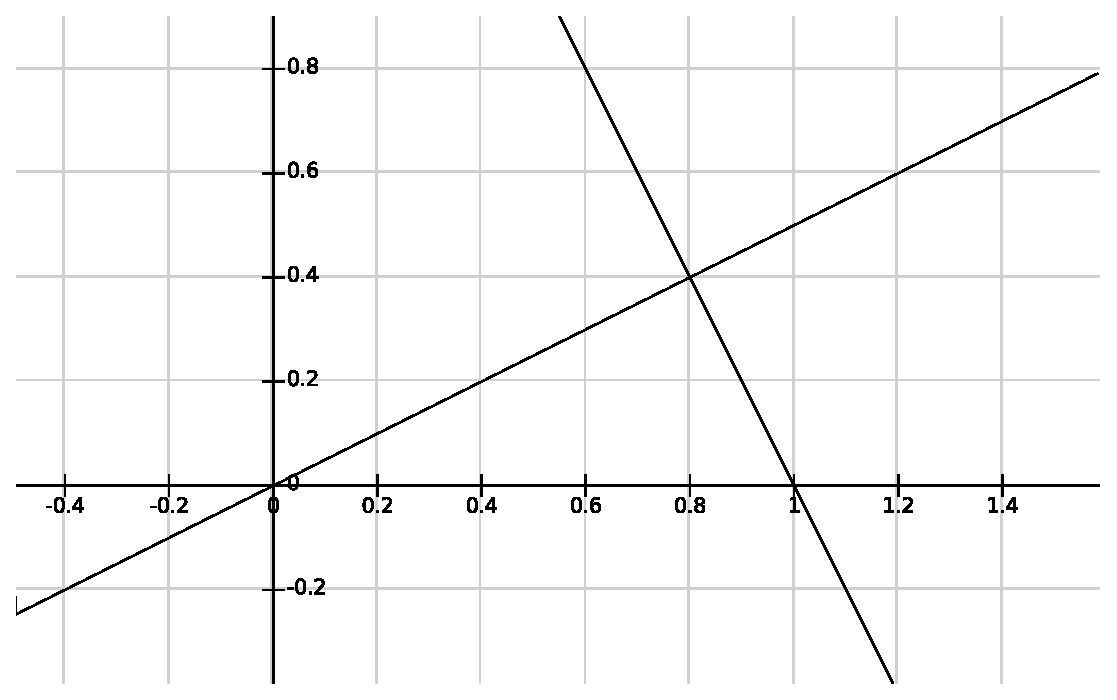
\includegraphics[width=0.5\textwidth]{a3.eps} 
  \caption{Function $w_2 = 0.5 w_1$ and $w_2 = -2 w_1 + 2$. The x-axis denotes $w_1$ and the y-axis denotes $w_2$.}
  \label{fig:q3.3}
\end{figure}
Figure \ref{fig:q3.3} shows the function of the gradient descent direction and the solution equation in part \textbf{3.3.1}. The crossing point is $w_1 = 0.8, w_2 = 0.4$.
\paragraph{3.3.3} \emph{Give a geometric argument that among all the solutions on the line, the gradient descent solution from the previous part has the smallest Euclidean norm.} \\
\\
See the Figure \ref{fig:q3.3} above, the line passing $(1, 0)$ is the solution line. The Euclidean norms of all the solutions are the distance between origin and the solution point. Therefore, the intersection, $(w_1 = 0.8, w_2=0.4)$, of the solution line and the line, which is perpendicular to the solution line and passing the origin and the solution point, is the optimal solution. Using Pythagorean theorem, we can find that the triangle formed by these two lines and the x-axis is a right-angled triangle, since the squares of the three sides are 1, 0.8, and 0.2.
\end{homeworkSection}
%%% Subquestion 4
\begin{homeworkSection}
\textbf{Overparameterized Model: General Case.}
\paragraph{3.4.1} \emph{Now we generalize the previous geometric insight developed to general $d > n$. Show that gradient descent from zero initialization i.e. $\hat{w}(0) = 0$ finds a unique minimizer if it converges. Write down the solution and show your work.} 
\\
\\
As we have
\begin{gather*}
\begin{aligned}
\frac{\partial L}{\partial \hat{w}} = \frac{2}{n} (X^TX\hat{w} - X^Tt) &= 0 \\
X^TX\hat{w} &= X^Tt \\
XX^TX\hat{w} &= XX^Tt \\
(XX^T)^{-1}XX^TX\hat{w} &= (XX^T)^{-1}XX^Tt \\
X\hat{w} &= t
%\quad \text{or} \quad \frac{\partial L}{\partial \hat{w}} = \frac{2}{n} \sum (\hat{w}^T x^{(i)} - t^{(i)}) x
\end{aligned}
\end{gather*}
Possible solutions are on hyperplane $X\hat{w} = t$. 
The iterative gradient descent equation is 
\begin{gather*}
\begin{aligned}
&\textbf{w}(0) \leftarrow \frac{\alpha}{n} \textbf{X}^T\textbf{t} \\
&\textbf{w} \leftarrow \textbf{w} - \frac{\alpha}{n} (\textbf{X}^T\textbf{X}\textbf{w} - \textbf{X}^T\textbf{t}) = \textbf{w} - \frac{\alpha}{n} \textbf{X}^T(\textbf{X}\textbf{w} - \textbf{t}) 
%\text{or} \quad & \textbf{w} \leftarrow \textbf{w} - \frac{\alpha}{n} \sum (\textbf{w}^T \textbf{x}^{(i)} - t^{(i)}) \textbf{x}^{(i)}
\end{aligned}
\end{gather*}
Thus, $\hat{w}$ can be written as 
\begin{gather*}
\begin{aligned}
\hat{w}=X^Td
\end{aligned}
\end{gather*}
where $d \in \mathbb{R}^n$. \\
To show the gradient descent from zero initialization finds a unique minimizer: 
\begin{gather*}
\begin{aligned}
X\hat{w} &= t \\
X X^T d &= t \\
d &= (XX^T)^{-1} t
\end{aligned}
\end{gather*}
Thus, 
\begin{gather*}
\begin{aligned}
\hat{w} &= X^T (XX^T)^{-1} t
\end{aligned}
\end{gather*}
\paragraph{3.4.2} \emph{Given the gradient descent solution from the previous part $\hat{w}$ and another zero-loss solution $\hat{w}$, evaluate $(\hat{w} - \hat{w}_1)^T\hat{w}$ .Use this quantity to show that among all the empirical risk minimizers for $d > n$, the gradient descent solution has the smallest Euclidean norm.} \\
\\
The gradient descent solution from the previous part is 
\begin{gather*}
\begin{aligned}
\hat{w} = X^T (XX^T)^{-1} t
\end{aligned}
\end{gather*}
and $\hat{w}_1$ is on hyperplane
\begin{gather*}
\begin{aligned}
X \hat{w}_1 = t \quad or \quad
\hat{w}_1^T X^T = t^T
\end{aligned}
\end{gather*}
then, we have
\begin{gather*}
\begin{aligned}
(\hat{w} - \hat{w}_1)^T \hat{w} &= (\hat{w}^T - \hat{w}_1^T) \hat{w} \\
&= \hat{w}^T\hat{w} - \hat{w}_1^T \hat{w} \\
&= t^T (XX^T)^{-1} X X^T (XX^T)^{-1} t - \hat{w}_1^T X^T (XX^T)^{-1} t \\
&= t^T (XX^T)^{-1} t - t^T (XX^T)^{-1} t \\
&= 0
\end{aligned}
\end{gather*}
The product between $\hat{w}$ and the difference between $\hat{w}$ and another zero-loss solution $\hat{w}$ is always 0, which means these two vectors are perpendicular. The norm of other solutions is larger than $\hat{w}$; thus, among all the empirical risk minimizers for $d > n$, the gradient descent solution has the smallest Euclidean norm.
\end{homeworkSection}
%%% Subquestion 4
\begin{homeworkSection}
\textbf{Benefit of Overparameterization.} \emph{Visualize and compare underparameterized with overparameterized polynomial regression.}
\begin{lstlisting}[language = PYTHON, keywordstyle=\color{blue!100}, 
    commentstyle=\color{red!50!green!50!blue!50}, 
    rulesepcolor=\color{red!20!green!20!blue!20}, 
    basicstyle=\small\ttfamily,
    breaklines=true,]
def fit_poly(X, d,):
    X_expand = poly_expand(X, d=d, poly_type = poly_type)
    if n > d:
        ## W = ... (Your solution for Part 3.2.1)
        W = np.linalg.inv(X_expand.T.dot(X_expand)).dot(X_expand.T).dot(t)
    else:
        ## W = ... (Your solution for Part 3.4.1)
        W = X_expand.T.dot(np.linalg.inv(X_expand.dot(X_expand.T))).dot(t)
  return W
\end{lstlisting}
\end{homeworkSection}
\end{homeworkProblem}

\end{document}

%\begin{gather*}
%\end{gather*}



